%=============================================================================
% SECTION 3 - The Demo Chain
%=============================================================================

% TODO maybe change title...
\section{The Demo Chain}
\label{sec:demo-chain}
In order to assess the performance of the MUSIC algorithm, an implementation
created by Ettus Research \cite{cite:ettus-doa} has been used. They provide an
application which proves the phase synchronization capability of their TwinRX
daughtercards, inside the GNU Radio framework. Figure \ref{fig:grc-fg} shows the
flow graph created with the GNU Radio Companion. \\

\begin{figure}[h]
    \centering
    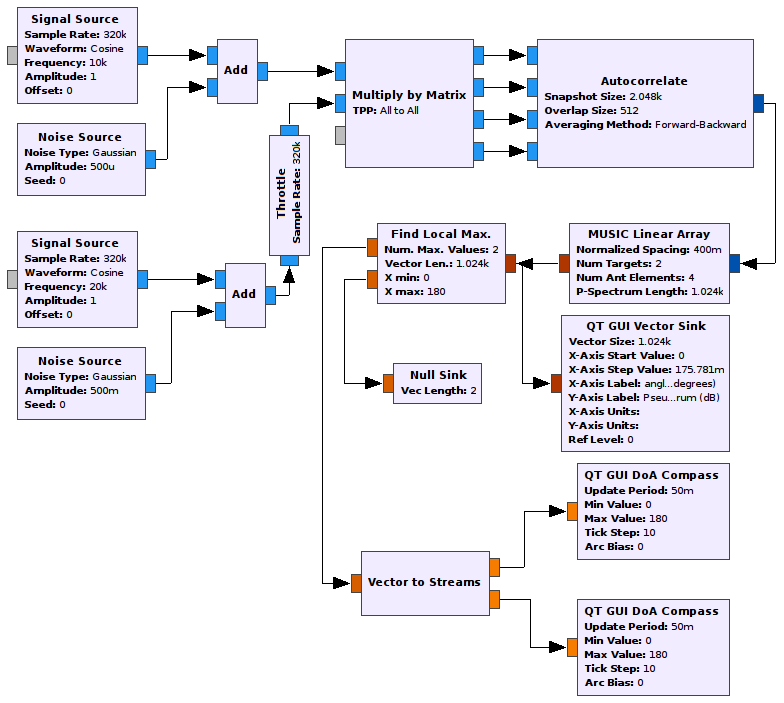
\includegraphics[width=\textwidth]{graph_doa}
    \caption{The flow graph used for the MUSIC algorithm}
    \label{fig:grc-fg}
\end{figure}


To explain the functionality of the graph, we need to define a set of
parameteres used in various block. The names of the parameters do not
necessarily reflect the actual names of the variables used in the code, but make
it easier to identify the parameters of interest. Also, some parameters are also
denoted by a shorter name, to make notations easier where it applies.
\begin{itemize}
  \item \code{sample\_rate} The rate at which the input signal is sampled
  \item \code{tone\_freq\_i} The frequency of the $i^{th}$ input signal
  \item \code{norm\_spacing} The normalised distance between the elements of the
  antenna array
  \item \code{num\_targets} The number of input signals, also denoted by N
  \item \code{num\_array\_elements} The number of elements in the antenna array,
  also denoted by M
  \item \code{p\_spectrum\_length} The length of the computed MUSIC spectrum
  \item \code{snapshot\_size} The number of samples used in computing the
  autocorrelation, also denoted by K
  \item \code{overlap\_size} The number of samples that overlap when computing
  successive values of the autocorrelation
\end{itemize}

\subsection{The input data}
This configuration uses two signal sources ($D = 2$) which generate cosines of
frequencies 10 kHz and 20 kHz, over which we add Gaussian noise, and an antenna
array with four elements ($M = 4$). The \textbf{Throttle} block is
used to limit the data throughput to the frequency of the input signal's
frequency, as it would behave in the case of a real signal arriving at an
antenna.

\subsection{The Multiply by Matrix block}
This block is used to simulate the way signals arrive at the antenna array, by
multiplying the array manifold matrix with an array which consists of samples of
the incoming signals. The general behaviour of the block is that if $\bm{A}$ is
the matrix that is given as a parameter to the block, of size M by N, and
$\bm{X}_N$ is a column array built from the $N$ inputs given to the block, then
the result of the multiplication is
\begin{equation}
\bm{Y}_M = \bm{A}\bm{X}_N,
\end{equation}
where $\bm{Y}_M$ is an column array constructed from the outputs of the block.
Thus, the block should have a number of N inputs and M outputs. \\

The array manifold matrix takes into account the angles of arrival and the
normalised distance between the elements of the array. The normalised spacing is
the distance between the antenna elements divided by the wavelength of the
carrier. According to \cite{cite:ettus-doa}, the normalised spacing should be at
most half of the center wavelength of the signal, otherwise aliasing could
interfere with the angle resolution performance of the MUSIC algorithm. \\

In our case, the array manifold matrix is:
\begin{displaymath}
    \begin{bmatrix}
        \bm{a}(\theta_1) & \bm{a}(\theta_2)
    \end{bmatrix}
\end{displaymath}
where $\bm{a}(\theta_i)$ is the steering vector corresponding to the angle of
arrival of the $i^{th}$ signal. The outputs of the \textbf{Multiply by Matrix}
block represent the sum of the signals that arrive at different angles at each
element of the antenna array.

% TODO find out why in the algorithm they use the autocorrelation rather then
% the autocovariance. it's just a normalization missing, but maybe it's
% important
\subsection{The Autocorrelate block}
The following block, \textbf{Autocorrelate}, corresponds to the step
\S1 of the MUSIC algorithm, although it actually computes an estimate of the
autocorrelation of the signal in the form of a sample correlation matrix. This
method implies collecting a sample over a snapshot time of the signal that
arrives at each element of the antenna array. Thus, an M by 1 array is formed,
denoted $x(k)$, and the sample correlation matrix is computed as follows:
\begin{equation}
C_x = \frac{1}{K}\sum_{k=1}^{K}\bm{x}(k)\bm{x}^H(k).
\end{equation}

Another method of computing the sample correlation matrix is collecting a number
of samples over a snapshot period denoted K, forming the matrix $\bm{X_K}$ of
dimensions N by K, which leads to the following formula:
\begin{equation}
C_x = \frac{1}{K}\bm{X_K}\bm{X_K}^H.
\label{eq:autocorr-first-part}
\end{equation}

In \cite{cite:FB-Averaging} it has been suggested that an additional step
consisting of a Forward-Backward Averaging of the sample correlation matrix will
increase the performance of the DoA estimation, so the computation can be
adjusted as such:
\begin{equation}
C_x = \frac{1}{2K}\bm{X_K}\bm{X_K}^H + \frac{1}{2K}\bm{J}\bm{X_K}^*\bm{X_K}^T\bm{J},
\end{equation}
where J is a reflection matrix (elements on the cross-diagonal are equal to 1
and the rest are 0). \\

The parameters of the \textbf{Autocorrelate} block are:
\begin{itemize}
    \item Snapshot size, previously denoted as K, representing the number of
    input samples used in computing the correlation matrix for an output item
    \item Overlap size, the number of samples that overlap in the computation
    for an output item to the next
    \item Averaging method, which can be either Forward-Backward or the standard
    Forward method
\end{itemize}

\subsection{The MUSIC Linear Array block}
In this application, we assume that we know the number of targets, so we do not
need a separate block to perform step \S2. Therefore we proceed directly to the
\textbf{MUSIC Linear Array} block, which computes the MUSIC spatial spectrum
from the step \S3. \\

In the constructor of the block, an array manifold vector is generated, which
uses a span of the possible angles between 0 and 180 degrees, with a resolution
of \code{1/d\_spectrum\_length}. The way the algorithm works, the closer an angle used
in generating the array manifold vector is to the actual angle of arrival, the
closer the MUSIC spectrum is to 0. In theory, when they coincide, the MUSIC
spectrum will reach 0. Therefore, for each input item a number of
\code{d\_spectrum\_length} values of the MUSIC spectrum have to be computed. \\

To compute the MUSIC spectrum, the block takes as input the result of the
autocorellation, on which an EigenValue Decomposition (EVD) is performed, and
then the desired spectrum is computed according to forumla
\eqref{eq:music-spectrum}. The block takes as parameters the number of targets,
the number elements in the antenna array and the normalised distance between
them, and also the spectrum length. \\

% TODO: why they take only the real part of Q_temp

\subsection{The Find Local Max block}
In order for the application to find the precise values of the angles of
arrival, a further block named \textbf{Find Local Max.} is needed, which solves
the step \S4 of the algorithm. The block outputs the coordinates (that is, the
angle) at which the peaks in the spectrum are found and looks precisely for $D$
such maximums. The block also gives information about the amplitude of the
spectrum at the given locations, but since they are of no importance for this
application, they are directed towards a \textbf{Null Sink}.

\subsection{Visualising the results}
We can either visualise the spectrum immediately after the \textbf{MUSIC Linear
Array} block, such as in Figure \ref{fig:doa-sp}, and form a good idea about the
estimated angle of arrival with the \textbf{QT GUI Vector Sink} block or, using
the \textbf{QT GUI DoA Compass} widget, we can see the estimated angle of
arrival for the two signals after we found the peaks in the spectrum. One
example of such an output for one of the signals can be found in Figure
\ref{fig:doa-compass}. Using two sliders, we can change the angle of arrivals in
real time and observe how the algorithm is adapting to the changes.

\begin{figure}[H]
    \centering
    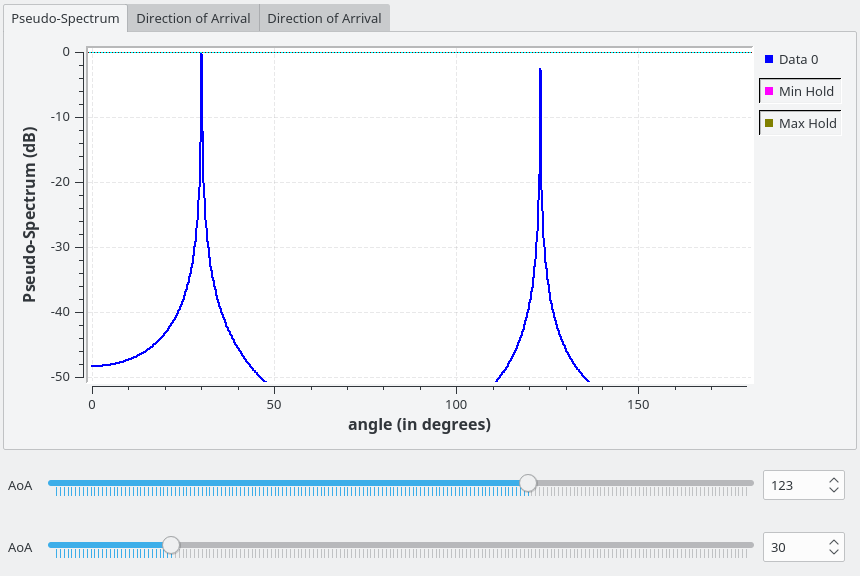
\includegraphics[width=0.75\textwidth]{grc-doa-spectrum}
    \caption{The MUSIC spectrum}
    \label{fig:doa-sp}
\end{figure}
\begin{figure}[H]
    \centering
    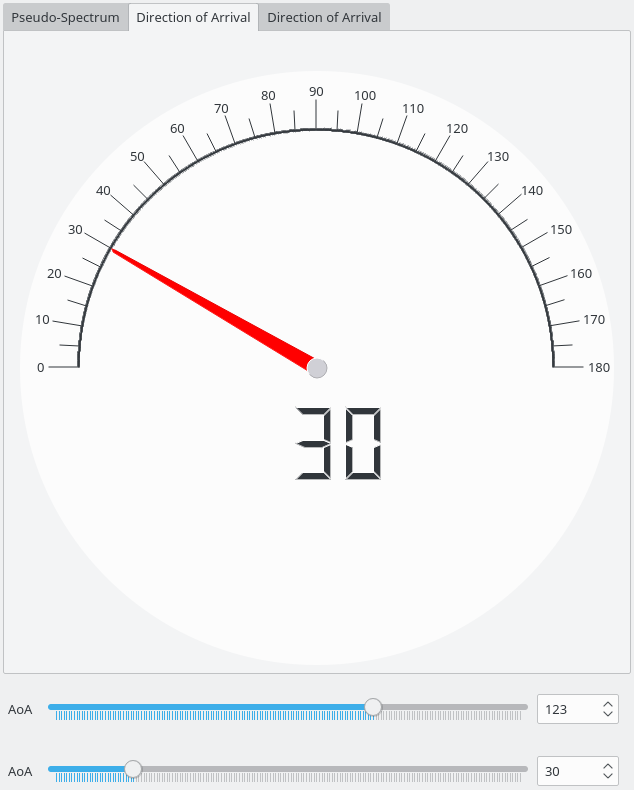
\includegraphics[width=0.4\textwidth]{grc-doa-compass}
    \caption{The estimated angle of arrival for one signal}
    \label{fig:doa-compass}
\end{figure}
